%------------------------------------------------------------------------------
\chapter{Irregular Sampling}
\vspace{-1cm} \label{cap3}

%\begin{flushright}
%\begin{minipage}{0.7\linewidth}
%\emph{``Quando uma criatura humana desperta para um grande sonho e
%sobre ele lan�a toda a for�a de sua alma, todo o universo conspira a
%seu favor.''}
%\end{minipage}
%\end{flushright}
%
%\begin{flushright}
%{Goethe}
%\end{flushright}

%\vspace{1cm}

%%Colocar uma descri��o do cap�tulo aqui!
%\section{Introdu��o}\label{sec int_cap_2}

In the last chapter, we  reviewed sensor fusion motivations, advantages and techniques. Despite all the growth and benefits from fusing data form multiple sensors, some challenges naturally appear. For the state estimation problem in sampled-data systems, a common challenge is related to sampling irregularities introduced in the network.

In this chapter, we review the irregular sampling problem. First, in Section \ref{sec:intro} we categorize the different types of irregularities that may occur in sampling and discuss their main causes and particularities. Then, in Secton~\ref{sec:irreg_types}, each irregularity is further discussed, with examples, mathematical models and their subdivisions, where applicable. We end this chapter with a discussion of time synchronization in Section~\ref{sec:sync}, which is needed to guarantee a common time scale for all nodes in network, enabling the irregularities to be dealt with appropriately.

\section{Introduction}\label{sec:intro}

Sampling irregularities may occur due to a variety of issues. Sometimes as undesired side effects of using large sensor networks architectures and others due to deliberate non-uniform sampling schemes. In this section we try to categorize and review the main irregularities observed in practice. The diagram in Figure \ref{fig:diagrama2} provides a simplified overview of them, separated by their sources.

\begin{figure}
\centering
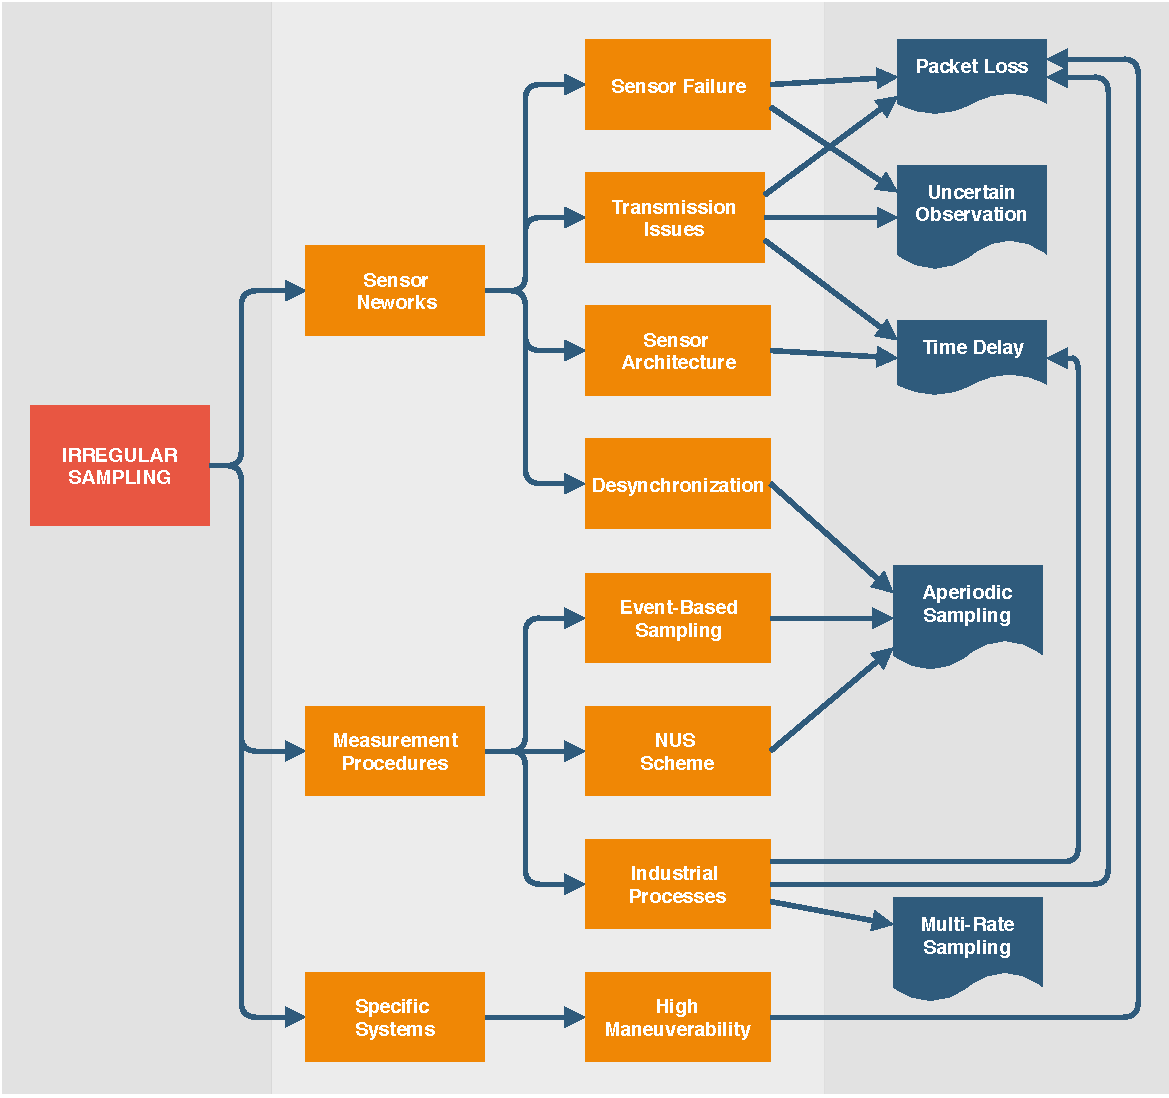
\includegraphics[width=0.85\textwidth]{Imagens/irreg_sampling.pdf}
\caption[Irregular sampling diagram]{Irregular sampling diagram, showing the main causes (in orange) and effects (in blue) of irregularities}
\label{fig:diagrama2}
\end{figure}

Networked system monitoring and control appears to be the main cause of irregular sampling. Unreliable communication channels may lead to random time delays and loss of information, specially if data are transmitted using a common media \citep{Sahebsara2007, Moayedi2011}. In case they get randomly interrupted during transmission or if a sensor fails at some point, the signal received may predominantly contain noise, causing uncertain observation or packet dropouts \citep{Hadidi1979, Wang2009}. Systems that are observed by a large number of desynchronized sensors will provide observations at random time intervals \citep{Micheli2002}. If they are synchronized but designed to operate in a centralized fashion, there is a chance that different time delays are produced due to distinct transmission routes for each sensor \citep{Bar-Shalom2000, Challa2003, Anxi2005}. 

However the communication networks shall not always be held responsible. Some applications are designed to be measured in an irregular way. In event-based schemes, for example, the measurements are transmitted only when certain conditions are met \citep{Liu2014,Zou2017}. Such approach can reduce communication resource consumption substantially \citep{Hu2017}, but will cause aperiodic sampling. Non-Uniform Sampling (NUS) is also intentionally used as an alias detection method \citep{Kunoh2015} or to enhance the spectral resolution of signals, largely used in Nuclear Magnetic Resonance (NMR) spectroscopy analysis \citep{Hyberts2013}. In other situations, due to the nature of the process being observed, the measurement strategy relies on different procedures. A lot of chemical processes, for instance, can be measured in an online, fast rate and delay free fashion, but provides inaccurate data. Therefore, lab analyses are used to improve estimation quality, but they are usually gathered at slower rates, sometimes irregularly and with possible time delays \citep{Fatehi2017}. Other industrial applications suffer from the same dilemma, and the sampling scheme ends up with a multi-rate data transmission, with random time delays and possibly measurement scarcity \citep{Penarrocha2012}. 

Finally, sampling irregularities might also appear due to a specific nature of a system. In some high maneuverable target-tracking applications, for example, there is a chance that the sensor misses the target, transmitting only noise, leading to the so called uncertain observation issue \citep{Wang2009, Chen2013}.

Whatever the reason for the irregularities, data need be associated in order to be fused into knowledge. A crucial part of association is temporal synchronization of observations, so that the exact time at which measurements are taken are available \citep{Ping2003}. Most sensor fusion methods for irregularly sampled systems rely on the correct time-stamps to 
develop modifications in classical algorithms. If observations are imprecisely time stamped, some alternatives have been proposed \citep{Julier2005, Huck2011} that incorporate some aspects of that imprecision in the estimation method. Still, some knowledge about the irregularity is assumed to be known. Alternatively, many techniques for time synchronization can be performed, to ensure a common time scale for all the sensors. 

On the next sections, we review the main irregular sampling effects and the main approaches to deal with time synchronization in sensor networks.

\section{Sampling Irregularity Types}\label{sec:irreg_types}
\subsection{Time Delay}

Time-delay systems (TDS) are probably the most common mathematical representation to time delays in practice. The works of \citep{Richard2003, Fridman2014} and the references therein provide a good coverage of the subject. In TDSs, there might be delays in the input or in the output signals, introduced by communication networks, or even in the states themselves. The latter phenomenon is called system with aftereffect or dead-time. Since we are studying the irregular sampling issue, only signal delays are relevant to us.

Considering delays in the measurement model only, \citep{Lu2005} studied the estimation problem when they are constant and known. They describe a linear measurement model as

\begin{equation}\label{eq:delay_model}
	y_i(t)=H_i(t)x(t_i)+v_i(t)
\end{equation}


\noindent
where $i=0,\ 1,\ ...,\ l$ and $l$ is the number of different known delays. $y_i(t) \in \mathbb{R}^{p_i}$ are delayed measurements and $v_i(t) \in \mathbb{R}^{p_i}$ the measurement noises. The known delayed time instants are given by $t_i=t_{i-1}-d_i$, with $d_0=0$, $d_i>0$ for $i>0$ and $t_0=t$. 

For some systems, delays might not be known and constant, but still multiple of a fixed value. In such cases, observations might be received in a burst, when more than one packet arrive between two consecutive sampling instants. When that happens, the estimator might use only the latest measurement and discard all others, or implement a buffer to iterate over all received packets \citep{Moayedi2011}.

However, in many applications the measurements are received by the estimator with irregular and unknown delays, although taken at regular time intervals. In such cases, time delays can be interpreted as a stochastic process $d(k)$, varying randomly throughout time. \citep{Han2009} describes a discrete-time measurement model for random delayed observations as

\begin{equation}\label{eq:delay_model2}
y(k) = H(k)x(k-d(k))+L(k)v(k)
\end{equation}

\noindent
where $d(k)$ is a random but bounded time delay, assumed to be a discrete-time Markov Chain observable at each sampling time $k$.

Multiple of a known lag or not, delayed measurements from a multisensor system are subject to arrive disordely, which leads to the sampling irregularity commonly known as out-of-sequence-measurements (OOSM). It can be classified in three ways, depending on the number of lags, according to Figure~\ref{fig:oosm}. 

\begin{figure}[!htb]
	\centering
	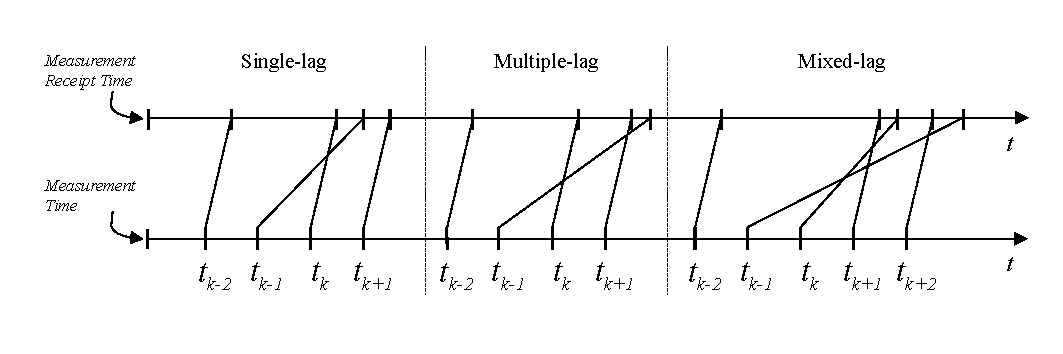
\includegraphics[width=0.85\textwidth]{Imagens/oosm.pdf}
	\caption{Different classes of out-of-sequence measurements irregularities}
	\label{fig:oosm}
\end{figure} 

\citep{Anxi2005} describes four different filtering approaches to deal with OOSM: reprocessing, that stores filter results to rollback with the time-delayed measurement; data buffering, that holds a set of measurements, greater than the maximum expected lag, to be sorted before filtering; discarding data, that neglects time-delayed measurements; and directly updating, that uses the delayed information to update current state estimate. \citep{Bar-Shalom2000} used the last approach to describe an optimal filter for the single-lag case.

A summary of causes and effects that time delay causes in an estimator are illustrated in Figure \ref{fig:diagrama_delay}.

\begin{figure}[!htb]
	\centering
	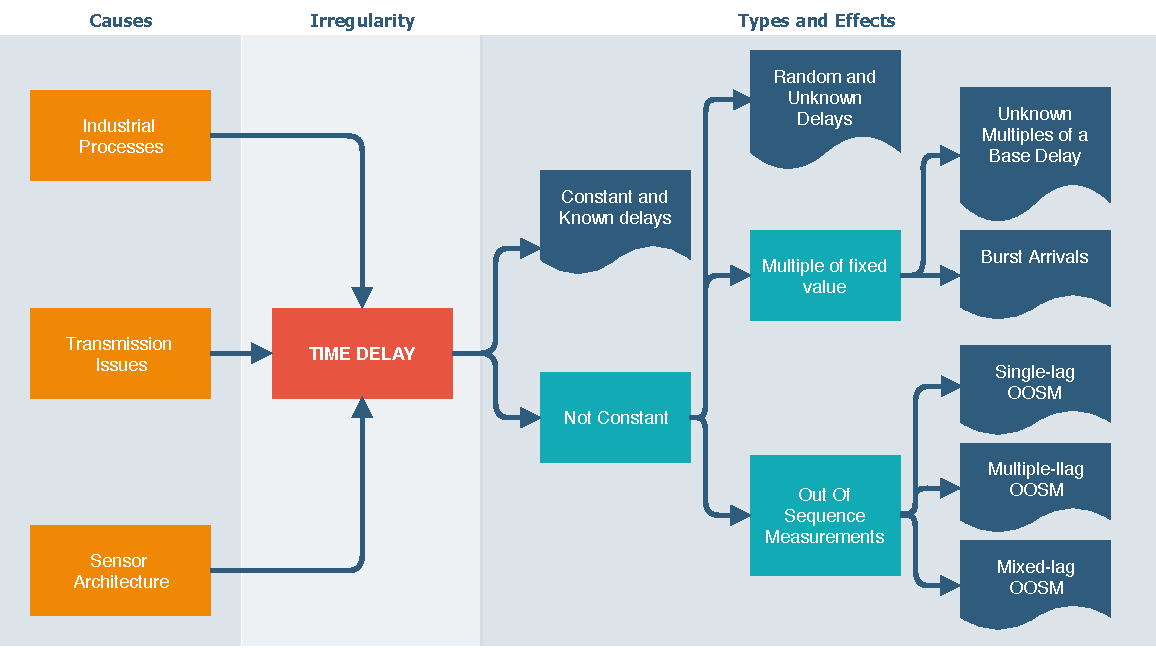
\includegraphics[width=0.75\textwidth]{Imagens/scheme_time-delay.pdf}
	\caption[Time delay diagram]{Time delay diagram, showing the main causes (in orange) and effects (in dark blue) of time delay irregularity. The light blue boxes indicate different types that lead to different effects.}
	\label{fig:diagrama_delay}
\end{figure}

\subsection{Packet Loss}

When data are being transmitted by a large network of sensors, there is a probability that they get lost in the way or they might arrive after a significant delay, which is equivalent to a loss for practical	 applications~\citep{Sinopoli2004}. Usually referred to as packet dropout/loss, missing/intermittent observations or scarse measurements~\citep{Albertos2004} they may happen due to node failures, network congestion, limited bandwidth or temporal failure. 
	
Mathematical description of packet dropouts can be carried out recursively, as described in~\citep{Sun2011}, by

\begin{equation}
\centering
\begin{split}
z(t) & = H(t)x(t)+v(t), \\
y(t) & = \xi(t)z(t)+(1-\xi(t))y(t-1),
\end{split}
\end{equation}

\noindent
where $z(t) \in \mathbf{R}^m$ is the measured output transmitted to the estimator, $v(t) \in \mathbf(R)^m$ is white noise, $y(t) \in \mathbf{R}^m$ is the measurement received by the estimator and $\xi(t) \sim Ber(p)$ is a Bernoulli random variable that takes the value 1 with probability $p$ and 0 with probability $1-p$. That is, when $\xi(t)$ is 1, there is no packet dropout. If $\xi(t)$ is 0, however, the latest output is used at current time, in a recursive fashion.

Another way of describing multiple packet dropouts is by limiting the amount of consecutive dropouts ~\citep{ShuliSun2008}, where the received measurements are defined by

\begin{equation}
\begin{split}
y(t) = 	& \xi(t)z(t) + (1-\xi(t))\xi(t-1)z(t-1)+...\\
		& + (1-\xi(t))(1-\xi(t-1))...(1-\xi(t-N+1))z(t-N), N \geq 1,\\
\end{split}
\end{equation}

Such a model dictates that the measurement used by the estimator will be only the most recent available, and the amount of missing observations is limited to $N$. This conclusion can be drawn by the fact that

\begin{equation}
\xi(t)+(1-\xi(t))\xi(t-1) + ... + (1-\xi(t))(1-\xi(t-1))...(1-\xi(t-N+1)) = 1.
\end{equation}

A summary of causes and effects that time delay causes in an estimator are illustrated in Figure \ref{fig:packet_loss}.

\begin{figure}[!htb]
	\centering
	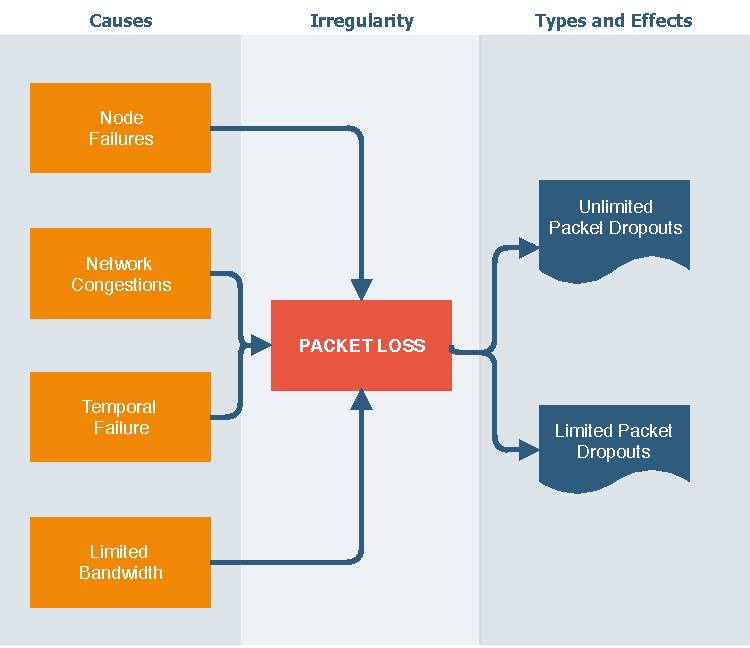
\includegraphics[width=0.75\textwidth]{Imagens/scheme_packet-loss.pdf}
	\caption[Packet loss diagram]{Packet loss diagram, showing the main causes (in orange) and effects (in dark blue) of time delay irregularity.}
	\label{fig:packet_loss}
\end{figure}


\subsection{Uncertain Observation}\label{sec:uncertain}

For some applications, there is a chance that the observation signal sent to the estimator contains only noise. According to \citep{Jaffer1971}, it happens as a consequence of two situations: the observation was taken, but was lost during transmission, due to communication failures; or it was not transmitted at all, as it may happen for target tracking systems, for example, when the object being observed is not tracked at a sample time. An observation model for a sampled-data system with uncertain observations can be described as

\begin{equation}
y(k) = \gamma(k)Cx(k) + Dv(k)
\end{equation}

\noindent
where $\gamma(k) \sim Ber(p(k))$ is a Bernoulli random variables, taking values of 0 or 1, with probabilities $p(k)$ and $1 - p(k)$, respectively.

Unlike the packet dropout problem, when the missing data are associated with the total absence of signal, the issue of uncertain observation has to be dealt with differently. A common approach is to detect the existence of signal prior to the assimilation, using a likelihood ratio test.  \citep{Middleton1968} proposes a joint approach to systematically detect and extract information from observation signals. If the estimator and detector are developed separately, the probability of false alarms is not used in the estimator, making it sub-optimal. \citep{Nahi1969} developed an optimal recursive estimator, that uses the information of the random variable $\gamma$ in the algorithm, assuming its sequence is independent and identically distributed. \citep{Hadidi1979} generalized the work of Nahi, for the case when the uncertainty of the signals presence is described by a Markovian sequence of binary random variables.

A summary of causes and effects that time delay causes in an estimator are illustrated in Figure \ref{fig:uncertain}.

\begin{figure}[!htb]
	\centering
	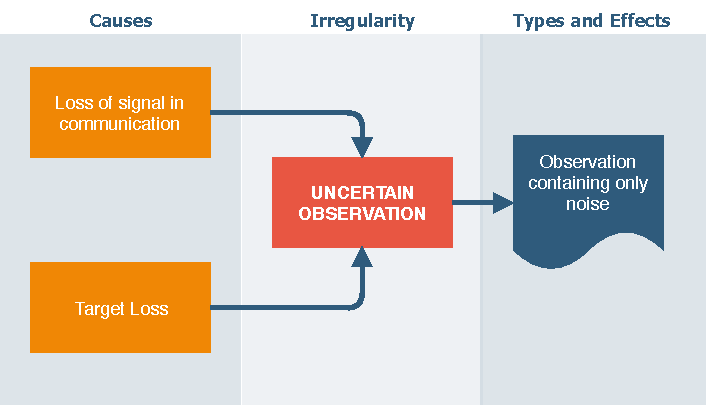
\includegraphics[width=0.75\textwidth]{Imagens/scheme_uncertain.pdf}
	\caption[Uncertain observations diagram]{Uncertain observations diagram, showing the main causes (in orange) and effects (in dark blue) of time delay irregularity.}
	\label{fig:uncertain}
\end{figure}

\subsection{Aperiodic Sampling}\label{sec:aperiodic}
	
All irregularities discussed so far may be present even in a periodic sampling scheme. However, for some applications, the sampling intervals are time-varying due to a variety of phenomena, causing the so called aperiodic or asynchronous sampling. It can be the case of networked and embedded control systems, with unpredictable networked-induced issues, like irregular faults on samplers, oscillated loads, intermittent saturation or even variations in system components or parameters \citep{Shen2016}. Some imperfections may cause what is known as sampling jitter noise, which leads to time intervals being almost uniform. Automotive applications, radar imaging or event controlled systems are a few examples. In them, jitter noise happens due to a sampling frequency similar to the clock frequency; to sampling requests delayed by the network; or to imperfect synchronization \citep{Eng2005}. For networks with a large amount of unsynchronized sensors, measurement arrival time instants are randomly spaced and can be modeled as a stochastic process \citep{Micheli2002}. Sometimes, the system being observed has particularities that causes the aperiodic sampling. One example is seismology, where the spatial coordinates are irregularly sampled, because of natural obstacles \citep{Marvasti2001}. Other large scale systems, such as power grids, have sensors with huge geographical separations and different communication links to the estimation hub, which causes multiple and random inter-observation intervals \citep{Yan2017}.

Whereas for most cases the deformities in sampling time intervals appear as unwanted effects, there are cases when the sampling rule is designed to work aperiodically. If there are limitations of communication resources (limited bandwidth or computation capacity) or a need for a reduced energy consumption, for example, time-driven sampling might be neglected in favor of an event-based scheme. In such strategy, an event-triggering mechanism is responsible for determining the sampling instants, according to Figure~\ref{fig:event-based}. For time-driven schemes, a clock triggers the transmission instants, while event-driven sampling instants depends on the sensor output itself with an optional feedback loop from the estimator, to assess estimation performance. Therefore, the trigger mechanism design provides a trade-off between performance and resource consumption efficiency, attracting a lot of research interest \citep{Liu2014}. The most common strategy for event-driven state estimation is the send-on-delta (SOD) \citep{Miskowicz2006}, which triggers the transmission when the value of the measured state deviates from the previous assimilated observation by an interval $\pm \Delta$, with $\Delta>0$. Other strategies were studied in \citep{Zou2017}. To avoid the risk of unexpected high amount of triggered measurements in a short period of time, which can lead to the dreaded Zeno behavior \citep{Tabuada2007}, lower-bounds can be defined both for the $\Delta$ value or for some explicit minimum inter-event time. 

\begin{figure}[!htb]
	\centering
	\begin{subfigure}
		\centering
		\text{(a)}\\
		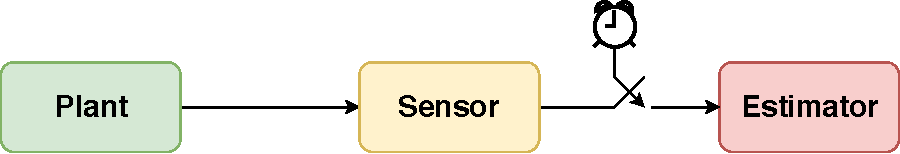
\includegraphics[width=0.75\textwidth]{Imagens/Event-based_clock.pdf}	
		\label{fig:evtb1}
	\end{subfigure}
	\vspace{1cm}\\
	\begin{subfigure}
		\centering
		\text{(b)}\\
		\vspace{0.25cm}
		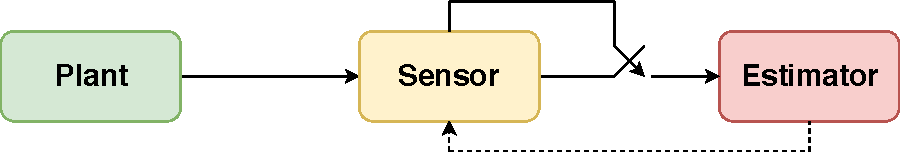
\includegraphics[width=0.75\textwidth]{Imagens/Event-based.pdf}
		%		\caption{}
		\label{fig:evtb2}
	\end{subfigure}
	\caption[Time-driven and event-driven sampling schemes]{Time-driven (a) and event-driven (b) sampling schemes. The connection between sensor and estimator is triggered by different mechanisms.}
	\label{fig:event-based}
\end{figure}

The measurement model of a linear system with aperiodic sampling can be defined as

\begin{equation}\label{eq:aperiodic}
y(t_k) = H(t_k)x(t_k) + v(t_k)
\end{equation}

\noindent
where $t_k$ is the random sampling time instant and the observation model matrix $H(t_k)$ is time-varying, if derived from the discretization of a continuous time system.

Generalizations of aperiodic sampling can be divided in two categories, based on how the estimator perceives the irregularity: as time noise added to a periodic pattern; or as a stochastic process, according to Figure~\ref{fig:aper-samp}. 

\begin{figure}[!htb]
	\centering
	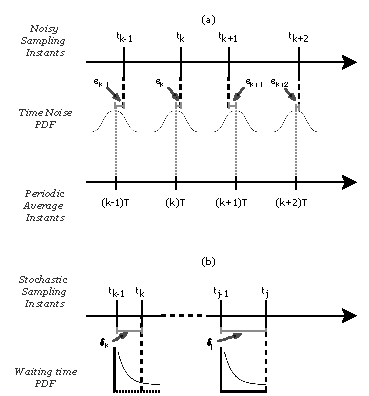
\includegraphics[width=0.85\textwidth]{Imagens/noisy_stoch_samp.pdf}	
	\caption[Aperiodic sampling categories]{Aperiodic sampling categories: (a) noisy sampling over periodic intervals, with a Gaussian random variable added to expected time instants $kT$; and (b) sampling instants modeled as a stochastic process, with time intervals characterized by an exponential random variable (cumulative distribution functions are shown, for different $\lambda$ parameter values.)}
	\label{fig:aper-samp}
\end{figure}

For the first case, random time instants $t_k$ and the random time intervals $\delta_k$ can be defined as:

\begin{equation}
\begin{split}
t_k & \triangleq kT + \epsilon_k, \\
\delta_k & \triangleq t_k - t_{k-1} 
\end{split}
\end{equation}

\noindent
where $t_k$ is the k\textsuperscript{th} sampling instant, $T$ is the periodic time interval and $\epsilon_k$ is the deviation from the expected value $kT$. Note that, if the sampling time instants are a sequence of i.i.d Gaussian random variables, with variance $\sigma^2$, that is $t_k \sim \mathcal{N} (kT, \sigma^2)$, $\forall k \sim \mathbb{N}$, then the time interval random variable is Gaussian, with expected value $T$ and variance $2\sigma^2$, that is $\delta_k \sim \mathcal{N}(T,2\sigma^2)$.

For the stochastic process generalization, sampling time instants $t_k$ can be defined by the random time intervals $\delta_k$, such as:

\begin{equation}
\begin{split}
\delta_k & \triangleq t_k - t_{k-1}, \\
\delta_0 & \triangleq t_1
\end{split}
\end{equation}

\noindent
where random time intervals $\delta_k$ can be modeled, in the most flexible way, as a gamma probability density function, that is $\delta_k \sim \Gamma(\kappa,\theta)$. If the shape parameter $k$ is a positive integer, it becomes an Erlang distribution, as used in \citep{Kanchanaharuthai2002}. For the most common case, where $\kappa$ is held constant, the random time interval $\delta_k$ follows an exponential PDF and the time sequence $t_k$ is represented by a Poisson stochastic process \citep{Micheli2002}. In fact, Micheli and Jordan provided mathematical proof that for a network with $N$ unsynchronized sensors with sampling period $T$, the waiting time between two arrivals tends, in distribution, to the exponential random variable, that is 
$\delta_k \sim \mathcal{E} (\lambda)$, where $\lambda = N/T$, as $N$ tends to infinity.

A summary of causes and types of aperodic sampling is presented Figure \ref{fig:aperiodic}.

\begin{figure}[!htb]
	\centering
	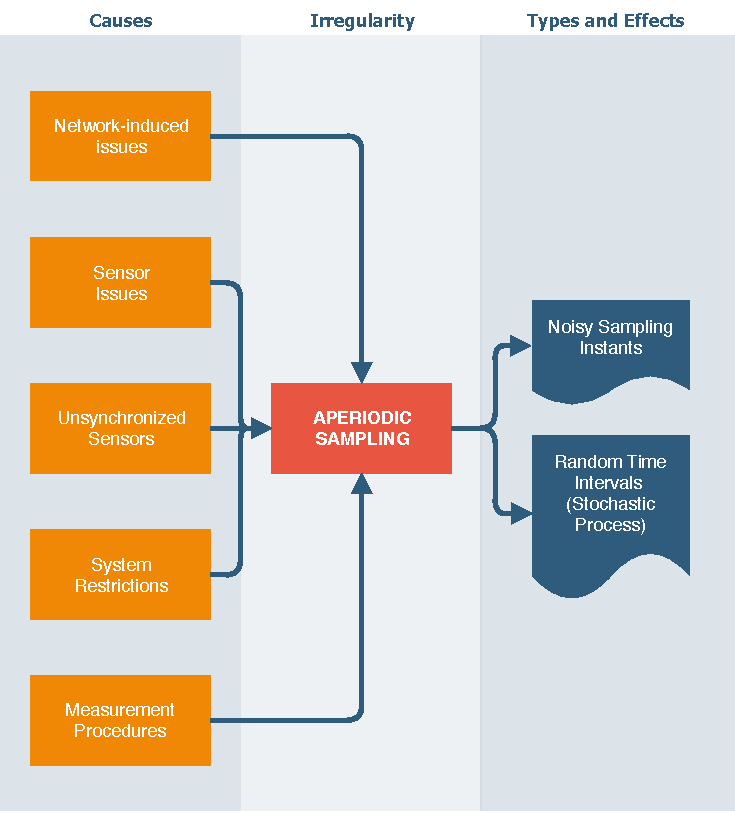
\includegraphics[width=0.75\textwidth]{Imagens/scheme_aperiodic.pdf}
	\caption[Aperiodic sampling diagram]{Aperiodic sampling diagram, showing the main causes (in orange) and types (in dark blue) of irregularity.}
	\label{fig:aperiodic}
\end{figure}

\subsection{Multi-Rate Sampling}

The last irregularity discussed is the multi-rate sampling. Generally, it refers to multiple sensors measuring the same system at different sampling rates. Many industrial processes need to control challenging variables that can be measured by online instruments that provide regular, fast rate and delay free information, but with low precision. Therefore, more accurate data are needed and usually available after slow, irregular and human-dependent laboratory analysis \citep{Penarrocha2012, Fatehi2017}. The combination of both sources of measurements leads to a multi-rate sampling scenario. 

A more common approach is the use of various sensors measuring the same physical information, to obtain better estimates, which has been drawing attention from real world applications, such as target tracking, robotics, surveillance and military. For such strategy, the sampling rates perceived by the estimator are often different from one another. The work of \citep{Lin2016} and the references therein provide a wide coverage of scenarios derived from multi-sensor multi-rate systems. 

Figure \ref{fig:multi-rate} illustrates the ways multi-rate sampling can be manifested in a system. The different rates from the various sensor devices can be periodic (a), aperiodic (b) or even a mixture of both, as it is the case for most industrial applications with laboratory analysis.

\begin{figure}[!htb]
	\centering
	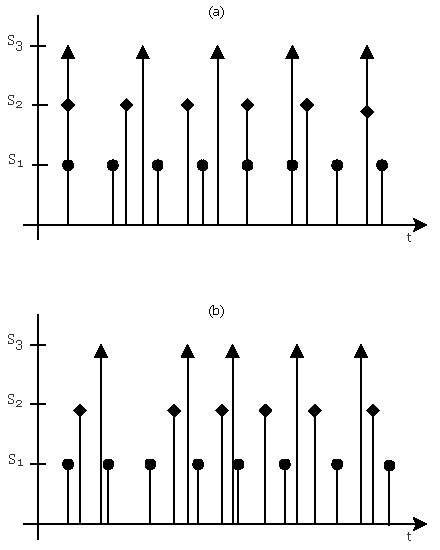
\includegraphics[width=0.5\textwidth]{Imagens/multi_rate.pdf}	
	\caption[Periodic and aperiodic multi-rate sampling scheme]{(a) Periodic and (b) aperiodic multi-rate sampling scheme. Labels $S_1$, $S_2$, $S_3$ refers to the sampling instants of three different sensors, from the highest rate to the lowest rate.}
	\label{fig:multi-rate}
\end{figure}

Aperiodic sampling rates can be described the same way as in Section \ref{sec:aperiodic}, by equation \ref{eq:aperiodic}. Periodic multi-rate measurements can be modeled as

\begin{equation}
	y_i(k_i) = H_i(x(k_i)) + v_i(k_1)
\end{equation}

\noindent
where $y_i(k_i)$ represents the $k_i^{th}$ observation from sensor $i$ and $H_i$ is the discrete measurement model matrix related to that sensor.

Figure \ref{fig:multi_rate} shows a schematic of causes and types of the multi-rate sampling irregularity.

\begin{figure}[!htb]
	\centering
	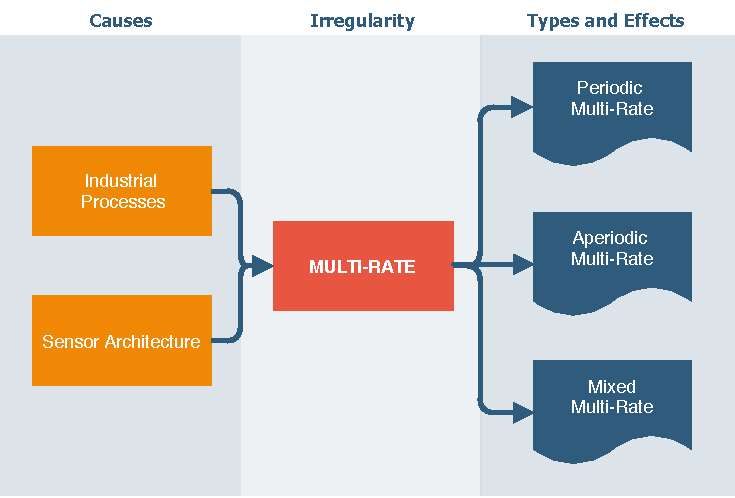
\includegraphics[width=0.75\textwidth]{Imagens/scheme_multi-rate.pdf}
	\caption[Multi-rate sampling diagram]{Multi-rate sampling diagram, showing the main causes (in orange) and types (in dark blue) of multi-rate sampling.}
	\label{fig:multi_rate}
\end{figure}


\section{Time Synchronization}\label{sec:sync}

There are techniques to handle all the irregularities discussed in this chapter and still achieve efficient state estimation performance. Provided that the estimator acknowledges the time that measurements were taken, there are many studies that propose different algorithms with interesting results. For some examples, we encourage the reader to check the references from each subsection in this chapter.

In general, multi-sensor data fusion techniques for state estimation require that exact measurement time-stamps are available in order to assimilate data properly \citep{Ping2003, Brahmi2013}. However, that is not always the case and situations may arise in which time-stamps were not collected or their values are unreliable. Examples of the latter may occur when measurements are time stamped when they are received by the estimator instead of the moment it was taken, or when they are time stamped at local clocks without centralized synchronization \citep{Julier2005}. 

<<<<<<< HEAD
In many practical applications, if sampling irregularity cannot be accounted for accordingly, data are fused using the time of arrival as time-stamp \citep{Huck2011}, or irregularities such as OOSM are just disregarded completely \citep{Kwok2004}. \citep{Julier2005} proved, however, that neglecting the uncertainty in time-stamp information may degrade estimation performance significantly in certain cases. They compared the results from traditional approaches that disregard or underestimate uncertain time stamps to algorithms that take the uncertainty statistics into account, knowingly: using fixed value for time instants derived from a calculated mean delay; a maximum likelihood algorithm for determining the predicted time measurement was taken; probabilistic data association filter (PDAF), proposed by \citep{Bar-shalom2009}; their approach, the Covariance Union (CU) algorithm; and the algorithm that uses the perfect time-stamp, to use as reference for the comparison. When irregularities happens in a situation where sensor information is sampled at much faster rates than filter update rates, the real-time particle filter (RTPF), proposed by \citep{Kwok2004}, makes efficient use of all sensor information, instead of discarding sensor readings. That is achieved by dividing the received measurements among sample sets and then representing the states as a mixture of those sets.
=======
In many practical applications, if sampling irregularity cannot be accounted for accordingly, data are fused using the time of arrival as time-stamp \citep{Huck2011}, or irregularities such as OOSM are just disregarded completely \citep{Kwok2004}. \citep{Julier2005} proved, however, that neglecting the uncertainty in time-stamp information may degrade estimation performance significantly in certain cases. For that, they compared the results from traditional approaches that disregard or underestimate uncertain time stamps to algorithms that take the uncertainty statistics into account, knowingly: using fixed value for time instants derived from an estimated mean delay; a maximum likelihood algorithm for determining the predicted time measurement was taken; probabilistic data association filter (PDAF), proposed by \citep{Bar-shalom2009}; their approach, the Covariance Union (CU) algorithm; and the algorithm that uses the perfect time-stamp, to use as reference for the comparison. When irregularities happens in a situation where sensor information is sampled at much faster rates than filter update rates, the real-time particle filter (RTPF), proposed by \citep{Kwok2004}, makes efficient use of all sensor information, instead of discarding sensor readings. That is achieved by dividing the received measurements among sample sets and then representing the states as a mixture of those sets.
>>>>>>> 2a6887ed554e336d3fc300055554e9075bb2e013

Alternatively, in order to avoid performance degradation, one can make use of time synchronization schemes, widely used in communication networks, to ensure global time stamps. Wireless sensor networks (WSN) are particularly dependent on such techniques, due to limited computation, energy and communication resources of the sensing devices used. The work of \citep{Sivrikaya2004} provide detailed reviews of the time synchronization problem in sensor networks. They explain the problem through computer clock mechanism. 

With the aid of a hardware oscillator, local clocks from a sensing device node $i$ approximates real time $t$ as $C_i(t)$ by
	
\begin{equation}\label{eq:clock1}
C_i(t) = a_it+b_i
\end{equation}

\noindent
where $a_i(t)$ is the clock \textit{drift}, that is the clock frequency, and $b_i(t)$ represents an \textit{offset} value, or the difference from real value $t$.

Clock approximations from two nodes in a network are compared by

\begin{equation}\label{eq:clock2}
C_1(t) = a_{12}C_2(t)+b_{12}
\end{equation}

\noindent
where $a_{12}$ is the relative \textit{drift} and $b_{12}$ is the relative offset between nodes. 

Under Equations~\ref{eq:clock1} and \ref{eq:clock2}, the synchronization problem becomes the equalization of the computer clocks from all different $n$ devices, in its most strict form. Thus, synchronization strategies can either match all clock frequencies and offsets once or perform repeated offset corrections over time. There are more relaxed versions of synchronizations, such as the one proposed by \cite{Roemer2003}, that aims at maintaining the order of events	only.	

Probably the most popular time synchronization method is the one being used in the internet environment for years, the Network Time Protocol (NTP), designed by \citep{Mills1991}. For most control and WNS applications, however, it is not suitable, due to very different requirements, such as energy consumption, precision and scalability \citep{Ganeriwal2003}. An easy solution would be to equip all sensing devices in the network with a global positioning system (GPS) for a global time synchronization, but such solution is very expensive, not energy efficient and its signal might not work properly in every environment.

Therefore, many alternative methods have been proposed, and the work of \citep{Kaur2015} updates Sivrikaya and Yener's studies with an exploration of the most recent synchronization protocols for sensor networks, that is: reference broadcast synchronization (RBS) \citep{Elson2002}; timing-sync protocol for sensor networks (TPSN) \citep{Ganeriwal2003};  delay measurement time synchronization (DMTS) \citep{Ping2003}; lightweight tree-based synchronization (LTS) \citep{Greunen2003}; tiny-sync mini-sync \citep{Sichitiu2003}; flooding time synchronization protocol (FTSP) \citep{Maroti2004}; lightweight and energy efficient time synchronization (LEETS) \citep{MingxiaXu2005}; time diffusion protocol (TDP) \citep{Su2005}; and time synchronization based on spanning tree (TSST) \citep{He2008}. A comparison adapted from Kaur ad Abhilasha is presented in Table~\ref{tab:sync}.


\begin{table}[!htb]
	\renewcommand{\arraystretch}{1.3}
	\caption[Comparison of time synchronization methods]{Comparison of time synchronization methods. Parameters are \textit{Precision, Energy Efficiency ($E.E.$) and Complexity ($Comp.$)}. Adapted from \citep{Kaur2015}}
	\label{tab:sync}
	\centering
	\begin{flushleft}
		
		{
			\footnotesize
			\begin{tabularx}{\linewidth}{
					>{\hsize=0.45\hsize}X
					>{\hsize=1.475\hsize}X
					>{\hsize=1.475\hsize}X
					>{\hsize=0.6\hsize}X}
				\hline
				\textbf{Protocol} 			& \textbf{Advantages}    			&  \textbf{Limitations} 		& \textbf{Parameters}\\ 
				\hline
				RBS & Eliminates random delays on the sender side & High amount of message exchanges and low transmission range & 29.1 $\mu s$ \ \ \ High $E.E.$ High $Comp.$ \\ \\
					
				TPSN & Eliminates the access, byte alignment and propagation times  & Does not estimate the clock drift; does not handle dynamic topology changes and demands high communication load & 16.9 $\mu s$ \ \ \ High $E.E.$ Low $Comp.$ \\ \\

				DMTS & Reduces the number of message exchanges  & Restricted to low resolution and low frequency external clocks & 32 $\mu s$ \ \ \ \ \ \ \ \ \ \ \ \ V. High $E.E.$ Low $Comp.$ \\ \\
					
				LTS & Robust and works well in the presence of dynamic links and fading.  & The accuracy of synchronization decreases linearly in the depth of the synchronization tree & Unknown \ \ \ Low $E.E.$ Low $Comp.$ \\ \\
									
				Tiny-Sync Mini-Sync & Tolerant to message losses and adequate for networks with limited bandwidth and computational power & Unsuited for mobile sensor networks, high convergence time, not scalable and little robustness & 945 $\mu s$ \ \ \ \ \ \ High $E.E.$ Low $Comp.$ \\ \\		
									
				FTSP & Robust, handles dynamic topology changes well and eliminates maximum delay components  & Does not eliminate propagation delay and is not scalable & 1.48 $\mu s$ \ \ \ High $E.E.$ High $Comp.$ \\ \\
										
				LEETS & Low power consumption and low amount of message exchanges & Requires a GPS receiver in the root node & 30 $\mu s$ \ \ \ \ \ \ \ 	High $E.E.$ Low $Comp.$ \\ \\
				
				TDP & Tolerant to message losses, high mobility and performs well even without external servers  & Very high convergence time & 100 $\mu s$ \ \ \ \ \ \ 	High $E.E.$ High $Comp.$ \\ \\
									
				TSST & Low synchronization error & Not scalable & Unknown  \ \ \ Low $E.E.$ Low $Comp.$ \\ \\
				
			\end{tabularx}
		}
	\end{flushleft}
\end{table}






\section{Chapter Summary and Final Remarks}

In this chapter, the main sampling irregularities are reviewed: time delay, packet loss, uncertain observation, aperiodic sampling and multi-rate sampling. Diagrams describing their causes, types and effects are shown for each of them. We also describe the necessary modifications to the observation models of state estimation algorithms. Most of the methods proposed in the literature to handle sampling irregularities rely on correct time stamping of observations. Thus, time synchronization in sensor networks becomes crucial and its further explored. The most recent protocols developed to ensure a global time scale from sensing devices in large sensor networks are shown and compared.

However, the use of any time synchronization method will require computational, energy and resource consumption to some extent, apart from complex algorithms implementations. For sensor fusion performance applications in state estimation of sampled-data systems with irregular sampling, the investment might not be worth it. Thus, the next chapters try to shed some light in the evaluation of performance degradation in state estimation in the presence of irregular sampling, if time-stamps are not available.


\clearpage